\documentclass[11pt]{article}

% ---------------- Packages ----------------
\usepackage[margin=1in]{geometry}
\usepackage{amsmath,amssymb,amsthm}
\usepackage{graphicx}
\usepackage{hyperref}
\usepackage{fancyhdr}
\usepackage{enumitem}
\usepackage[UTF8]{ctex}

% ---------------- Header ----------------
\pagestyle{fancy}
\fancyhf{}
\lhead{Course Name}
\rhead{Homework \#1}
\cfoot{\thepage}

% ---------------- Title ----------------
\title{Homework 1}
\author{羊瑞 \\ 2300013091}
\date{\today}

% ---------------- Custom commands ----------------
\newcommand{\R}{\mathbb{R}}
\newcommand{\E}{\mathbb{E}}

% ---------------- Problem Environment ----------------
\newcounter{problem}

\newenvironment{problem}[1][]{
\stepcounter{problem}
\section*{Problem \theproblem\; #1}
}{}

\newenvironment{solution}{
\par\noindent\textbf{Solution.}\par\noindent
}{\qed}

\setlength{\parindent}{0pt}
% ---------------- Document ----------------
\begin{document}

\maketitle

\begin{problem} 
\begin{center}
    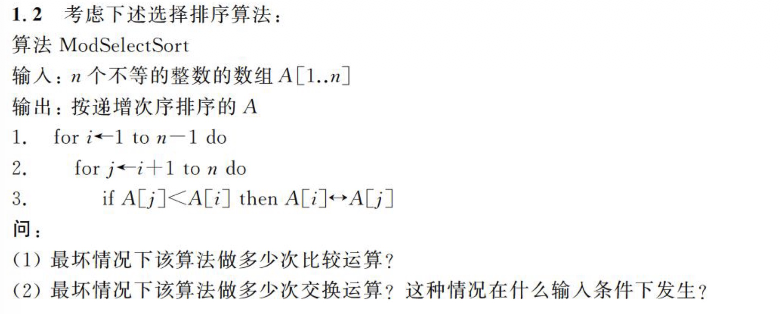
\includegraphics[width=0.6\textwidth]{problems/1-2.png}
\end{center}
\end{problem}

\begin{solution}

(1)最坏情况下比较次数为： $W(n) = 1+2+...+(n-1) = \frac{n(n-1)}{2}$. \\
(2)最坏情况下, 交换次数与比较次数相等, 为 $\frac{n(n-1)}{2}$ 次, 此时输入的n个数从前到后严格单调递减.
\end{solution}

\begin{problem}
\begin{center}
    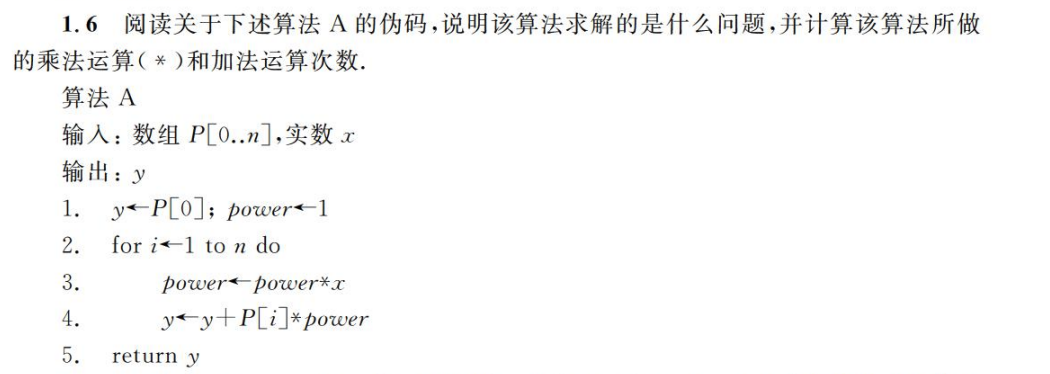
\includegraphics[width=0.6\textwidth]{problems/1-6.png}
\end{center}
\end{problem}

\begin{solution}

该算法求的是多项式 $P(x) = P[0] + P[1]*x + P[2]*x^2 + ... + P[n]*x^n$的值, 乘法运算次数2n, 加法次数n.
\end{solution}

\begin{problem}
\begin{center}
    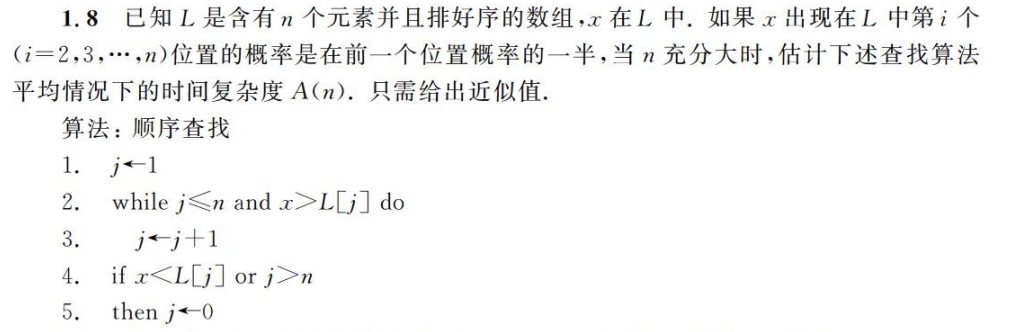
\includegraphics[width=0.6\textwidth]{problems/1-8.png}
\end{center}
\end{problem}

\begin{solution}

设x出现在第一个位置的概率为p, 则 $1 = p + \frac{p}{2} + \frac{p}{2^2} + ... + \frac{p}{2^n} + ...$, 故 $p = \frac{1}{2}$. \\
设算法结束所需次数为随机变量K, 有 $P(K <= k) = p + \frac{p}{2} + ... + \frac{p}{2^{k-1}} = \frac{1}{2} + \frac{1}{4} +... + \frac{1}{2^k} $, 进而 $P(K = k) = \frac{1}{2^k}$. \\
$A(n) = \frac{1}{2}*1 + \frac{1}{4}*2 + \frac{1}{8}*3 + ... + \frac{1}{2^n}*n \approx \frac{1}{2}*4 = 2 $.
\end{solution}

\begin{problem}
\begin{center}
    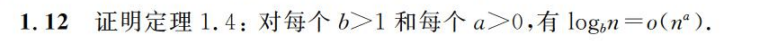
\includegraphics[width=0.6\textwidth]{problems/1-12.png}
\end{center}
\end{problem}

\begin{solution}

证明：$ lim_{n \to \infty} \frac{\log_b n}{n^a} = lim_{n \to \infty} \frac{\frac{1}{n\log b}}{an^{a-1}} = lim_{n \to \infty} \frac{1}{a\log b}\frac{1}{n^a} = 0 $, 所以 $\log_b n = o(n^a)$.
\end{solution}

\begin{problem}
\begin{center}
    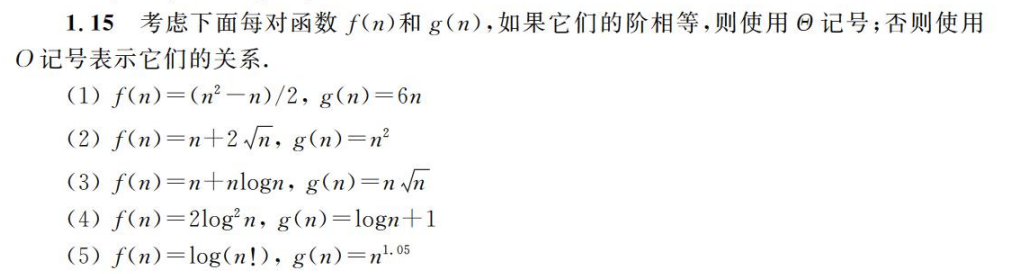
\includegraphics[width=0.6\textwidth]{problems/1-15.png}
\end{center}
\end{problem}

\begin{solution}

(2)$f(n) = O(g(n)) $ \\
(4)$g(n) = O(f(n)) $
\end{solution}

\begin{problem}
\begin{center}
    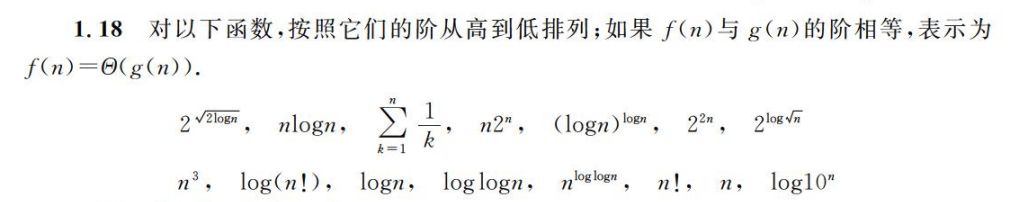
\includegraphics[width=0.6\textwidth]{problems/1-18.png}
\end{center}
\end{problem}

\begin{solution}

将函数按阶从高到低排列：\\
$n!, 2^{2n}, n2^n, n^{\log\log n} = \Theta((\log n)^{\log n}), n^3, n\log n = \Theta{\log (n!)}, n = \Theta(\log 10^n), 2^{log \sqrt{n}}, 2^{\sqrt{2\log n}}, \log n = \Theta({\sum_{k=1}^n} \frac{1}{k}), \log \log n $
\end{solution}

\begin{problem}
\begin{center}
    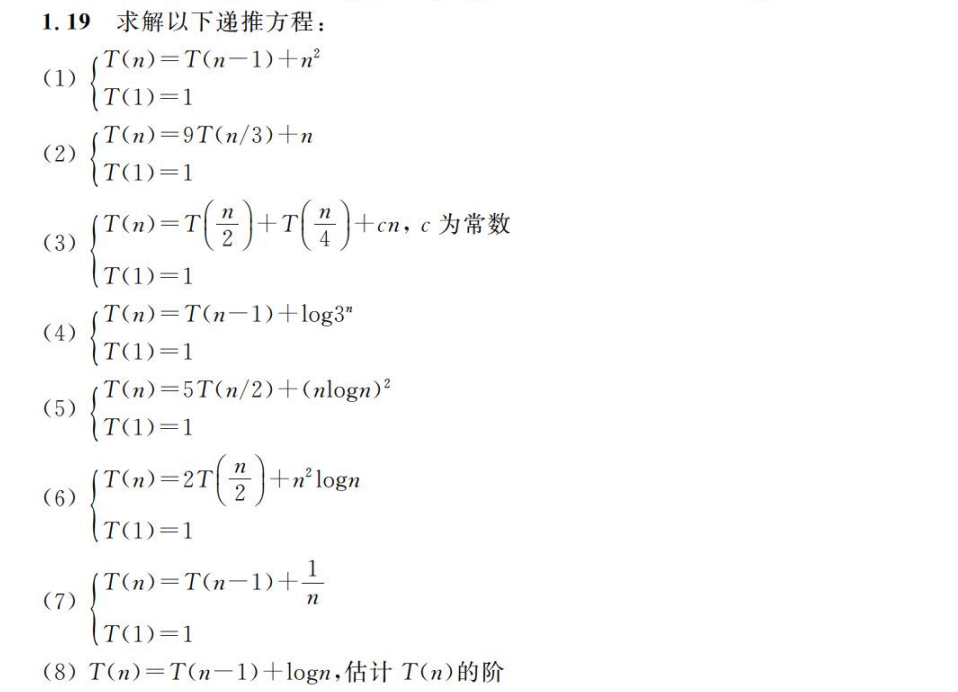
\includegraphics[width=0.6\textwidth]{problems/1-19.png}
\end{center}
\end{problem}

\begin{solution}

(2)带入主定理: $a=9, b=3, f(n) = n. n^{\log_b a} = n^2 $. f(n)阶更低, 所以 $T(n) = \Theta(n^2) $ \\
(4)$T(n) = T(n-1) + \log 3^n = T(n-2) + \log 3^n + \log 3^{n-1} = ... = n\log3 + (n-1)\log3 + ... + 2log3 + 1 = \Theta(n^2) $ \\
(6)带入主定理: $a = 2, b = 2, f(n) = n^2\log n. n^{\log_b a} = n $. f(n)的阶更高, $af(\frac{n}{b}) = 2f(\frac{n}{2}) = 2(\frac{n}{2})^2 \log \frac{n}{2} = \frac{n^2}{2}(\log n-1) <= \frac{n^2}{2}\log n <= \frac{1}{2}f(n) $. 取$c = \frac{1}{2}$满足条件. 所以 $T(n) = \Theta(n^2\log n)$.
\end{solution}

\begin{problem}
\begin{center}
    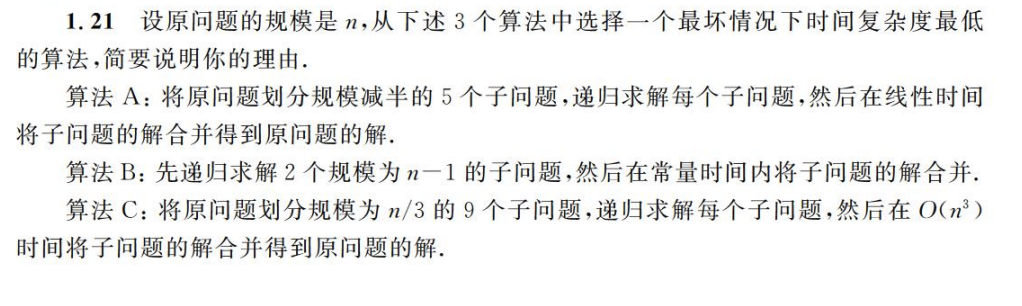
\includegraphics[width=0.6\textwidth]{problems/1-21.png}
\end{center}
\end{problem}

\begin{solution}

A: $T(n) = 5T(\frac{n}{2}) + O(n), T(n) = \Theta(n^{log_2 5}) $ \\
B: $T(n) = 2T(n-1) + O(1), T(n) = \Theta(2^n) $ \\
C: $T(n) = 9T(\frac{n}{3}) + O(n^3), T(n) = \Theta(n^3) $ \\
综上, 选择A.
\end{solution}

\end{document}